% Zylinderkondensator: Gauß-Zylinder (Radius r, Länge L) und E(r) ~ 1/r
% Gemeinsamer Stil für alle Abbildungen (TikZ -> SVG, siehe figures/build.mjs).
%
% Farben sind Platzhalter ("Sentinels"): build.mjs ersetzt sie im SVG durch
% CSS-Variablen, damit die Abbildungen im hellen und dunklen Modus passen.
% Andere Farben (auch schwarz/weiß) bricht der Build mit Fehler ab.
%
%   fg    Linien, Beschriftung          -> --dark
%   mu    Hilfslinien, Achsen, Maße      -> --gray
%   acc   das eine Konzept der Abbildung -> --secondary (Lime/Oliv)
%   blue  zweite Größe, negative Ladung  -> --fig-blue
%   warm  dritte Größe, positive Ladung  -> --fig-warm
%   bg    Seitenhintergrund (Aussparen)  -> --light
%
% Kein \clip verwenden: pdftocairo macht daraus Clip-Gruppen, in denen exakt
% waagerechte/senkrechte Linien verschwinden. Berechnete Kurven schneidet
% gen/*.py selbst am Rahmen ab.
\documentclass[tikz,border=3pt]{standalone}
\usepackage{amsmath,amssymb,bm}
% Text serifenlos wie die Seite, Mathe in Computer Modern wie KaTeX
\renewcommand{\familydefault}{\sfdefault}
\usetikzlibrary{arrows.meta,calc,decorations.markings,patterns,3d,positioning,angles,quotes}

\definecolor{fg}{RGB}{1,2,3}
\definecolor{mu}{RGB}{4,5,6}
\definecolor{acc}{RGB}{7,8,9}
\definecolor{blue}{RGB}{10,11,12}
\definecolor{warm}{RGB}{13,14,15}
\definecolor{bg}{RGB}{16,17,18}

% Vektoren wie auf der Website (KaTeX \mathbf)
\newcommand{\vv}[1]{\mathbf{#1}}

\tikzset{
  every picture/.style={fg, line width=0.8pt, line cap=round, line join=round,
    >={Stealth[length=5.5pt,width=4.4pt]}},
  every node/.style={font=\small},
  % Linientypen
  main/.style={line width=0.9pt},
  thin/.style={line width=0.5pt},
  aux/.style={mu, line width=0.5pt, dash pattern=on 2.5pt off 2pt},
  axis/.style={mu, line width=0.6pt, ->},
  vec/.style={line width=1.1pt, ->},
  field/.style={line width=0.7pt, postaction={decorate},
    decoration={markings, mark=at position #1 with {\arrow{Stealth[length=4.5pt,width=3.6pt]}}}},
  field/.default=0.5,
  % Flächen
  soft/.style={fill=#1, fill opacity=0.14},
  soft/.default=acc,
  % Ladungen
  qpos/.style={circle, fill=warm, inner sep=0pt, minimum size=9pt,
    path picture={\draw[bg, line width=0.9pt] ($(path picture bounding box.center)+(-2pt,0)$) -- +(4pt,0)
      ($(path picture bounding box.center)+(0,-2pt)$) -- +(0,4pt);}},
  qneg/.style={circle, fill=blue, inner sep=0pt, minimum size=9pt,
    path picture={\draw[bg, line width=0.9pt] ($(path picture bounding box.center)+(-2pt,0)$) -- +(4pt,0);}},
  dot/.style={circle, fill=fg, inner sep=0pt, minimum size=3pt},
  % Beschriftung mit Aussparung, damit Linien den Text nicht kreuzen
  lbl/.style={fill=bg, inner sep=1.5pt},
  % Icons: kräftigere Linien, keine Schrift
  icon/.style={line width=1.6pt, >={Stealth[length=6pt,width=5pt]}},
}

\begin{document}
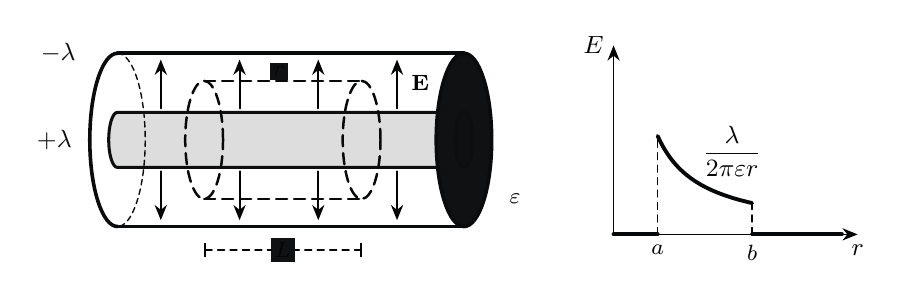
\begin{tikzpicture}
  \def\a{0.35} \def\b{1.1} \def\rg{0.75} \def\len{4.4} \def\e{0.32} % e: Ellipsen-Stauchung
  % Außenleiter (hinten: gestrichelte linke Hälfte der rechten Stirnfläche entfällt)
  \draw[blue, line width=1.3pt] (0,\b) -- (\len,\b) (0,-\b) -- (\len,-\b);
  \draw[blue, line width=1.3pt] (0,-\b) arc[start angle=270, end angle=90, x radius=\e*\b, y radius=\b];
  \draw[blue, thin, dash pattern=on 2pt off 1.5pt] (0,\b) arc[start angle=90, end angle=-90, x radius=\e*\b, y radius=\b];
  % Innenleiter
  \draw[warm, line width=1.1pt, soft=warm] (0,\a) -- (\len,\a) arc[start angle=90, end angle=-90, x radius=\e*\a, y radius=\a] -- (0,-\a)
    arc[start angle=270, end angle=90, x radius=\e*\a, y radius=\a];
  % radiales Feld in der Zeichenebene: senkrecht zur Achse, durchsetzt den Gauß-Zylinder
  \foreach \x in {0.55,1.55,2.55,3.55} {
    \draw[vec, line width=0.75pt] (\x,\a+0.05) -- (\x,\b-0.08);
    \draw[vec, line width=0.75pt] (\x,-\a-0.05) -- (\x,-\b+0.08);
  }
  \node[anchor=west, font=\footnotesize] at (3.6,0.72) {$\vv E$};
  % Gauß-Zylinder
  \begin{scope}[acc, line width=0.9pt, dash pattern=on 4pt off 2.5pt]
    \draw (1.1,\rg) -- (3.1,\rg) (1.1,-\rg) -- (3.1,-\rg);
    \draw (1.1,0) ellipse ({\e*\rg} and {\rg});
    \draw (3.1,0) ellipse ({\e*\rg} and {\rg});
  \end{scope}
  \node[acc, anchor=south, lbl, inner sep=1pt] at (2.05,\rg) {$r$};
  \draw[aux, |-|] (1.1,-\b-0.3) -- node[lbl, text=mu, font=\footnotesize] {$L$} (3.1,-\b-0.3);
  % Stirnfläche rechts mit radialem Feld
  \draw[blue, line width=1.3pt, fill=bg] (\len,0) ellipse ({\e*\b} and {\b});
  \draw[warm, line width=1.1pt, fill=warm, fill opacity=0.25] (\len,0) ellipse ({\e*\a} and {\a});
  \draw[warm, line width=1.1pt] (\len,0) ellipse ({\e*\a} and {\a});
  \node[warm, anchor=east] at (-0.45,0) {$+\lambda$};
  \node[blue, anchor=east] at (-0.4,\b) {$-\lambda$};
  \node[mu, font=\footnotesize, anchor=west] at (\len+0.45,-0.75) {$\varepsilon$};
  % Verlauf E(r)
  \begin{scope}[xshift=6.3cm, yshift=-1.2cm]
    \draw[axis] (0,0) -- (3.1,0) node[anchor=north, text=fg] {$r$};
    \draw[axis] (0,0) -- (0,2.4) node[anchor=east, text=fg] {$E$};
    \def\s{0.7}
    \draw[acc, line width=1.4pt] (0,0) -- (\a*1.6,0);
    \draw[acc, line width=1.4pt, domain=\a*1.6:\b*1.6, samples=50] plot (\x,{\s/\x});
    \draw[acc, line width=1.4pt] (\b*1.6,0) -- (2.9,0);
    \draw[aux] (\a*1.6,0) -- (\a*1.6,{\s/(\a*1.6)});
    \draw[aux] (\b*1.6,0) -- (\b*1.6,{\s/(\b*1.6)});
    \node[anchor=north, font=\footnotesize] at (\a*1.6,0) {$a$};
    \node[anchor=north, font=\footnotesize] at (\b*1.6,0) {$b$};
    \node[acc, anchor=west] at (1.0,1.05) {$\dfrac{\lambda}{2\pi\varepsilon r}$};
  \end{scope}
\end{tikzpicture}
\end{document}
